\section{Visual Design}

The design of system is driven by tasks, to align the analysis of mobility patterns with individual characteristics characteristics. Before diving into the design of system, we introduce the couple of specifical tasks the system intended for. 

\begin{itemize}
\item \textit{Task 1: Identify the group with specific individual characteristics}: to get groups of people with common or close attributes, to explore the correlation among individual characteristics.
\item \textit{Task 2: Explore the mobility patterns of a group}: to explore where, how and why an interested group go in city. 
\item \textit{Task 3: Compare mobility patterns among multiple groups}: to know the similarities and differences between different groups in their mobility patterns, to investigate the relationship between movement and individual characteristics.
\end{itemize}

\subsection{Design Considerations}

With these three tasks, we derive following design considerations:

\begin{itemize}
\item \textit{Effective multivarible cross-filter for individual characteristics (C1)}: there are eight domains to describe an individual. The system is supposed to provide a straright-forward way for easy filtering by the eight criteria.
\item \textit{Good overview of the multivarible individuals (C2)}: following the visual analytics manta by Shneiderman~\cite{RN459}, it is very important to provide a good overview of all the individuals then the users know where to explore. 
\item \textit{Intuitive perception of an individual as an organic complex (C3)}: the system should make use of users' daily life experience in knowing people to provide intuitive visualization, instead of the lifeless representation by number. The visual design needs to help end-users to pick desirable ones from the mass.  
\item \textit{Compact visualization of mobility patterns in the constraint of spatial space (C4)}: the analysis of mobility patterns not only includes the conventional spatial and temporal dimensions, but also other abstract dimensions, e.g., travel purpose, visiting frequency, etc. The system should handle a compact layout to support the easy correlation between spatial and abstract information. 
\item \textit{Flexible interactions to explore the mobility patterns either within one group or between groups (C5)}: to support the comparison among groups, \textit{Task 3}, the system should maintains flexbile interactions which allows the end-users to explore freely.
\end{itemize}

% Classification method, flow clustering method, Semantic representation. 

With those design considerations, we develop a visual analytics system as Figure~\ref{fig:teaser} shows. It composes of individual panel to explore and identify groups (\textit{Task 1}) and spatial panel to explore and compare the mobility pattern (\textit{Task 2 and 3}). \m{EXPAND..., it gives an infographical overview of the data. Encode information but also allow users to set multiple criteria (\textit{C1}). Support users to slice the data by different domains.}
% Semantic understanding of social characteristics.


\subsection{Data-driven Profile Visualization}

Glyph-based visualization~\cite{borgo2013glyph} is the form of visual design to compose multivaribles into a collection of unified visual symbols, known as glyph. Glyph is intended for quick understanding and aligned comparison. Among glyph design, Chernoff Face~\cite{chernoff1973use} represents data variabules by the different features of a cartoon face. Following the idea of Chernoff Face, we design a type of glyph, a graphical representation of people with specific individual characteristics. The idea behind using faces is that humans easily recognize faces and notice small changes without difficulty (\textit{C3}). Those visual profiles are intended for intutive visual understanding, from abstract to concrete and semantic understanding, to support users to target the interested individual groups effectively.

Figure~\ref{fig:design_profile} shows the legend for the user profile. The eight domains are encoded by visual symbols and organically organized in a human figure. There are bascially three types of variables to drive the figure, i.e., the numeric, categorical and boolean ones. For numeric attributes such as income and education levels, visual symbol keeps consistent design but with changing visual variation, such as size, thickness. For the categorical attributes such as job, visual symbols are designed seperately for better semantic meaning. For the boolean attribute like car, house, a symbol is designed to indicate its existence. With this consideration, the domains are designed as following:

% For numeric attributes. 

% By different composition, stimulus pattern which has the abstract deomgraphic measurement of individuals.

\begin{itemize}
\item \textbf{Gender} the gender is visually mapped to the hair style of the avatar. 
\item \textbf{Age} age is implied by the decoration on the hair. For the elder above 70, the hair is dyed to gray. For the youth beneath 18, a hair decoration is adapted for the different hair styles of girls and boys.
\item \textbf{Education} The thickness of eye glasses is used to indicate the different levels in education.
\item \textbf{Job} The clothes is designed to imply the job of the individual. There are 9 types of clothes.
\item \textbf{Belongings} for real estate, car, residential license are considered as the belongings to the individual, so we design each of them as an add-on decoration to imply whether the individual has it or not.
\item \textbf{Income} a money symbol is used to represent the income, whose size encodes the income level. The more money an individual earns, the larger the symbol is.
\end{itemize} 

\begin{figure}[htb!]
 \centering % avoid the use of \begin{center}...\end{center} and use \centering instead (more compact)
 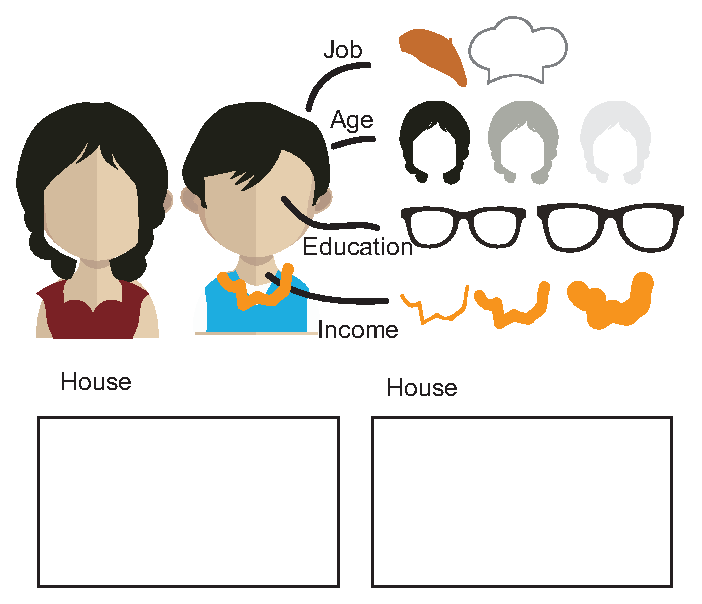
\includegraphics[width=\columnwidth]{pictures/design_profile}
 \caption{Design Profile: the eight characteritical domains are encoded and organized in an organic human figure.}
 \label{fig:design_profile}
\end{figure}

With the visual mapping, the profile varies from individual to individual. By concretizing the attributes which otherwise is too abstract to percept, users can scan and search for interesting target effectively. Figure~\ref{fig:div_example} lists the figures with the top 10 largest population in some job. The textual number beneath indicates the population. It is found that the majority of workmen earn low salary and most of them have no residential license. On the contrary, for the officers, all of them have residential license and most of them has house. Some of the retired people are in old age. Most of managers are at undergraduates, even graduates. 

% \begin{figure}[htb!]
%  \centering % avoid the use of \begin{center}...\end{center} and use \centering instead (more compact)
%  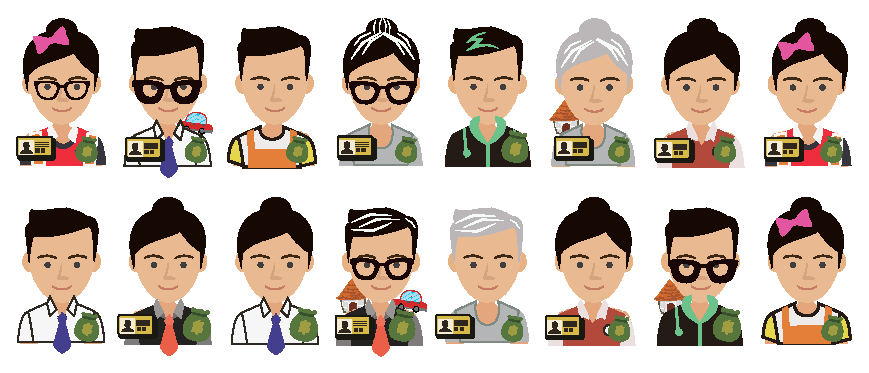
\includegraphics[width=\columnwidth]{pictures/design_div}
%  \caption{Diverse Profile}
%  \label{fig:div_profile}
% \end{figure}

 
\begin{figure}[htb!]
 \centering % avoid the use of \begin{center}...\end{center} and use \centering instead (more compact)
 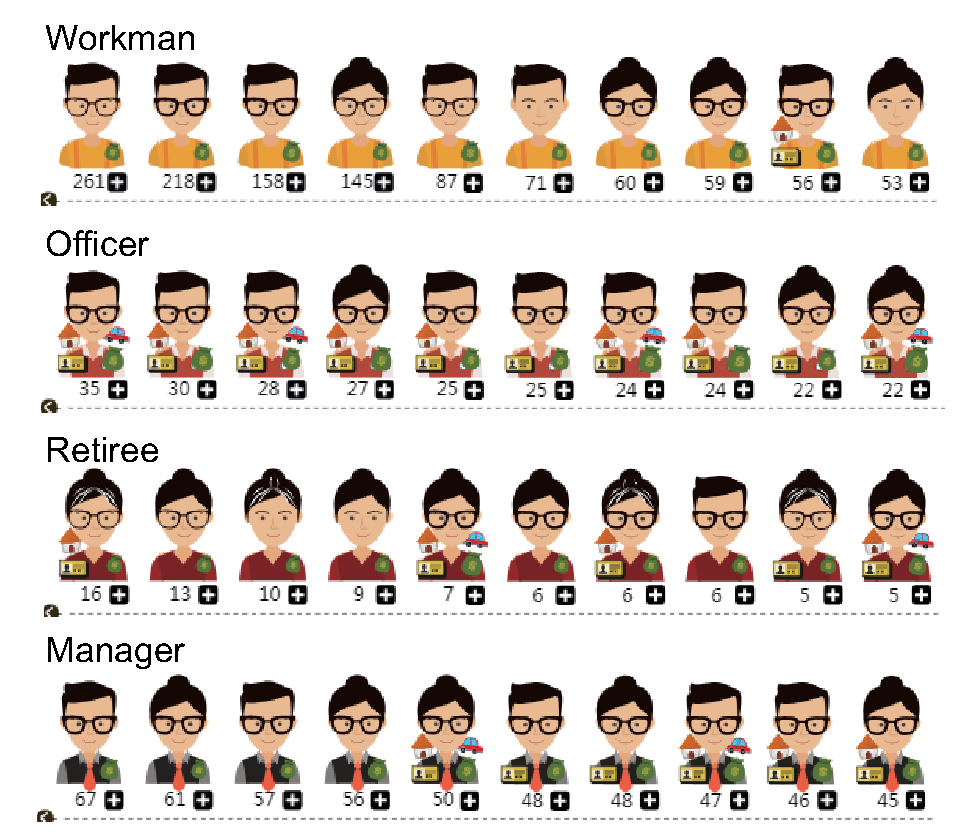
\includegraphics[width=\columnwidth]{pictures/design_example}
 \caption{Representative figures with the top 10 largest population in four jobs}
 \label{fig:div_example}
\end{figure}

\subsection{t-SNE Projection of Individuals}



% \begin{figure}[htb!]
%  \centering % avoid the use of \begin{center}...\end{center} and use \centering instead (more compact)
%  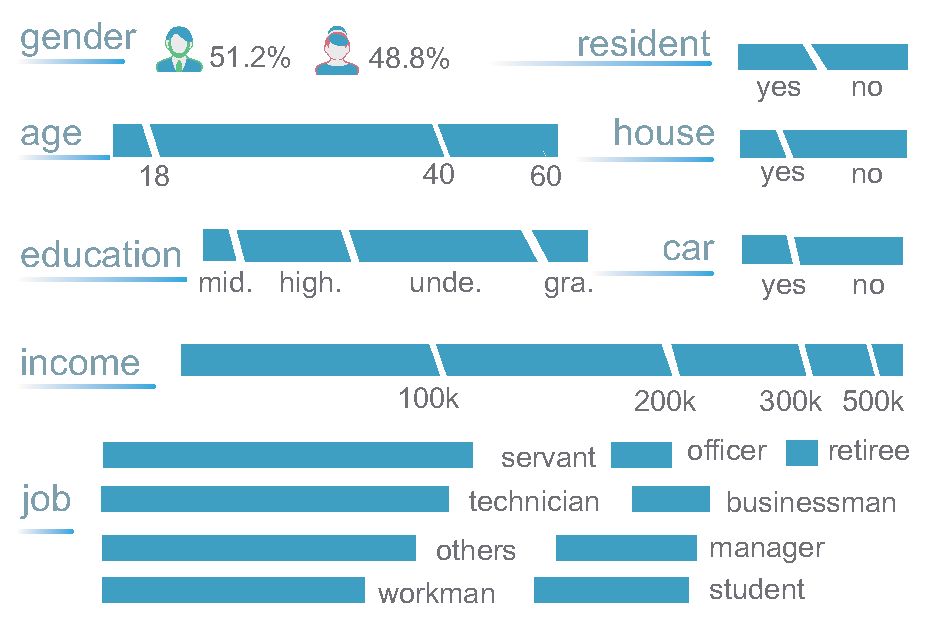
\includegraphics[width=0.7\columnwidth]{pictures/data_overview}
%  \caption{Overview of Multiple Variables}
%  \label{fig:figoverview}
% \end{figure}

In our case, each individual can be denoted as a vector $x_i$ with eight factors, and we get high dimensional data set $X={x_1, x_2, ..., x_n}$. The dimensionality reduction techniques are to preserve the local structure of high dimensional data in low dimensional space, which are efficient approaches to provide a good overview of the multivarible individuals. We adapt t-SNE project~\cite{maaten2008visualizing} to project $X$ as two-dimensional dots $Y={y_1, y_2, ..., y_n}$. 

t-SNE computes the conditional probabilities to represent the similarity based on the distance between high dimenional datapoints. The conditional probability $p_{j\mid i}$ between $x_j$ and $x_i$ is given by:

\begin{equation}
p_{j\mid i} = \frac{exp({\left \| x_i - x_j \right \|}^2/2\alpha_i ^{2})}{\sum _{k\neq i}exp({\left \| x_i - x_k \right \|}^2/2\alpha_i ^{2})}
\end{equation}



 which well suits high-dimensional data for visualization in a low-dimensional space of two dimensions (\textit{C2}). 

As Figure~\ref{fig:tsne}(a)shows, all volunteers are embedded evenly in the 2D view, indicating the uniformly sampling over demographical space. 

Multiple views of abstract view, t-SNE proection and semantic data driven profile visualization are coordinated in a Cross-filter machinesm~\cite{Weaver2010}. It allows end-users to interactive drill-down into individuals with interested characteristics from multiple perspectives. Starting from the abstract criterion constraints, the scope of interest is narrowed down to individuals with(out) certian properties. And then further cross-filtering with semantically visual profiles, to check the combination of 8 characteristical variables. Figure~\ref{fig:tsne}(b) examplifies four groups of interest. 

\begin{figure}[htb!]
 \centering % avoid the use of \begin{center}...\end{center} and use \centering instead (more compact)
 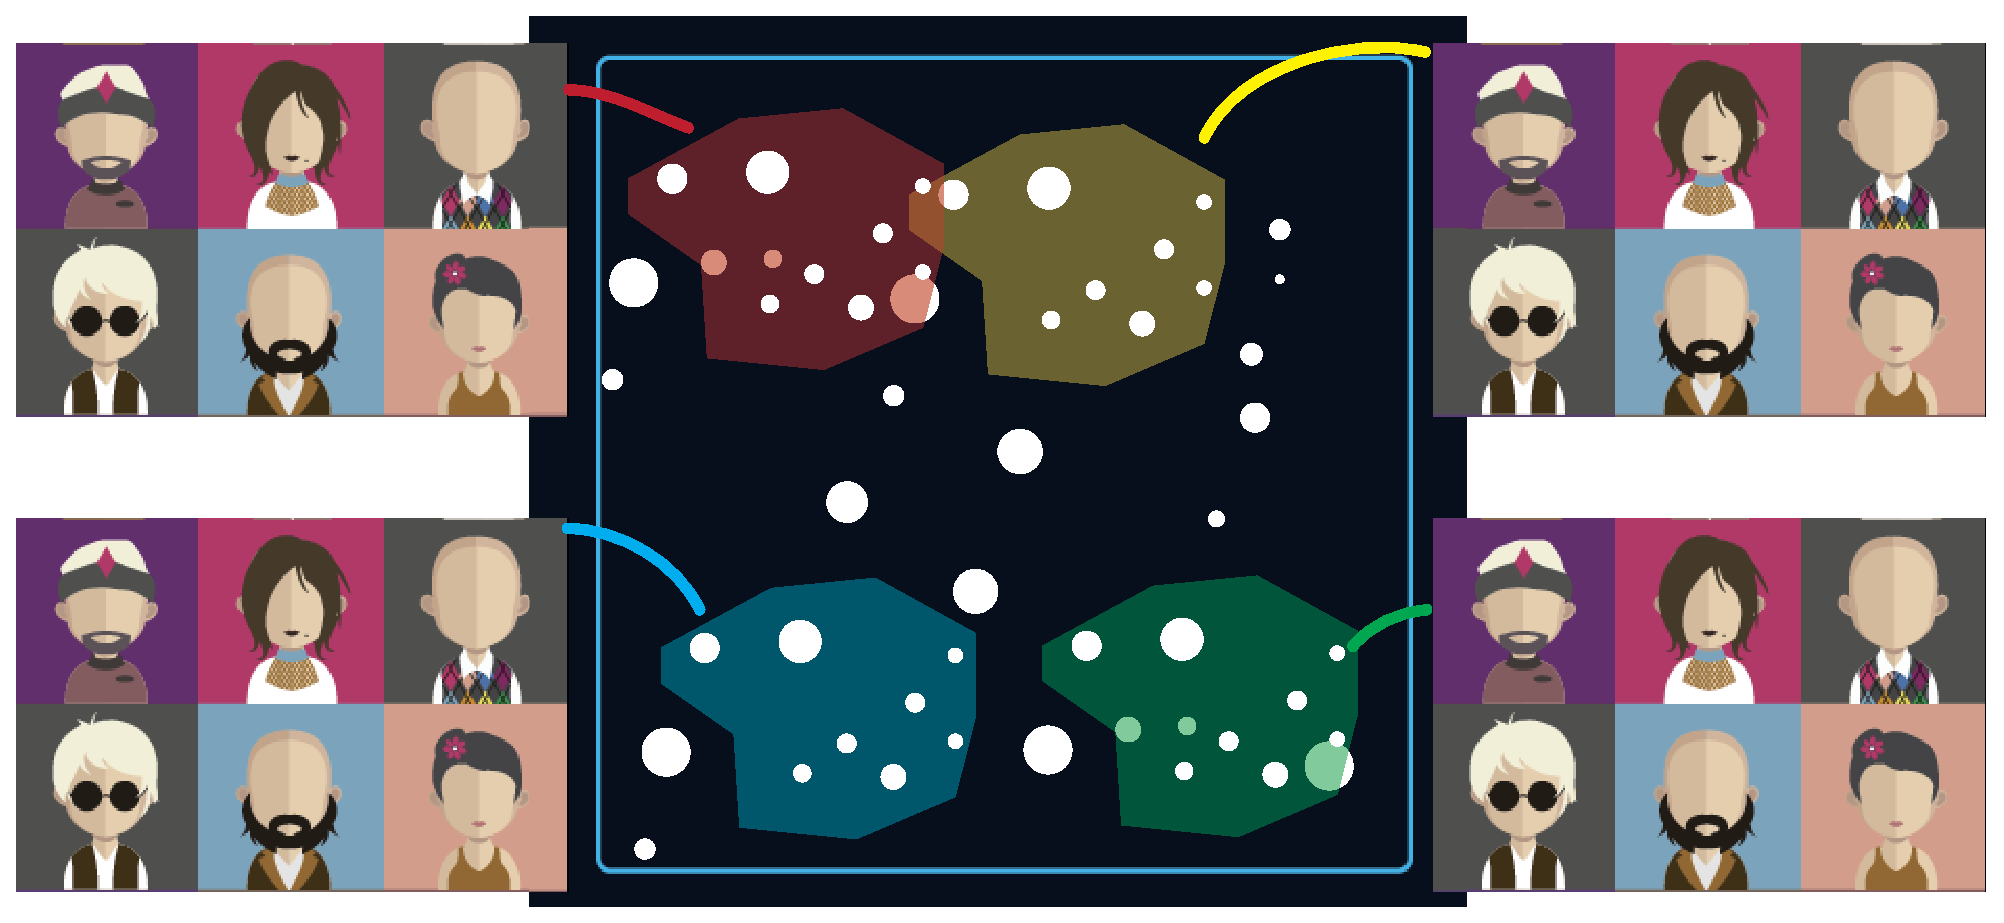
\includegraphics[width=\columnwidth]{pictures/mds}
 \caption{t-SNE project with four groups of the interest}
 \label{fig:tsne}
\end{figure}


\subsection{2.5D Spatial Visualization}

Embedding multiple variables in the spatial map is a challenging problem. Distortion technique 2D spatial, such as the partial route embedding~\cite{sun2016embedding}. However, when it comes to the global visualization, the trade-off between occlusion-free and the spatial perception. Follow the idea of 2.5D space design~\cite{Tominski2012_stacking}, the space visualization is embedded in 2.5D space, which also can smoothly transited back to the conventional 2D view.  

 Each TAZ is grown as a prism whose height encodes the occurrence of visiting. Brunch of TAZ with similar visiting pattern and purpose are grouped by an heuristic DB-Scan Algorithm in the context of TAZ. From a center TAZ, walk to neighbour TAZ to check whether aggregation or not. The aggregated TAZ brunch indicates the region visiting by the group of people in same purpose, which is often the popular traveling places. The TAZ brunch is visualized...

 To compare the mobility patterns across different groups of people, a Small Multiple dock is used to reserve the ever explored interesting result. To simply the comparion over spatial distribution, the snapshot is rendered in the 2D space, which can be magnified to check for the details in the 2.5D space.

 In this view, it supports end-users to direct manipulate the space, e.g., zooming, panning, etc. Also, detail information about the visiting can be checked by direct clicking on the TAZ. 